% Additional Technical Information
\newpage
\begin{landscape}
\section{Additional Technical Information}\label{sec:appC}
\subsection{Schematics}

\begin{figure}[h!]
	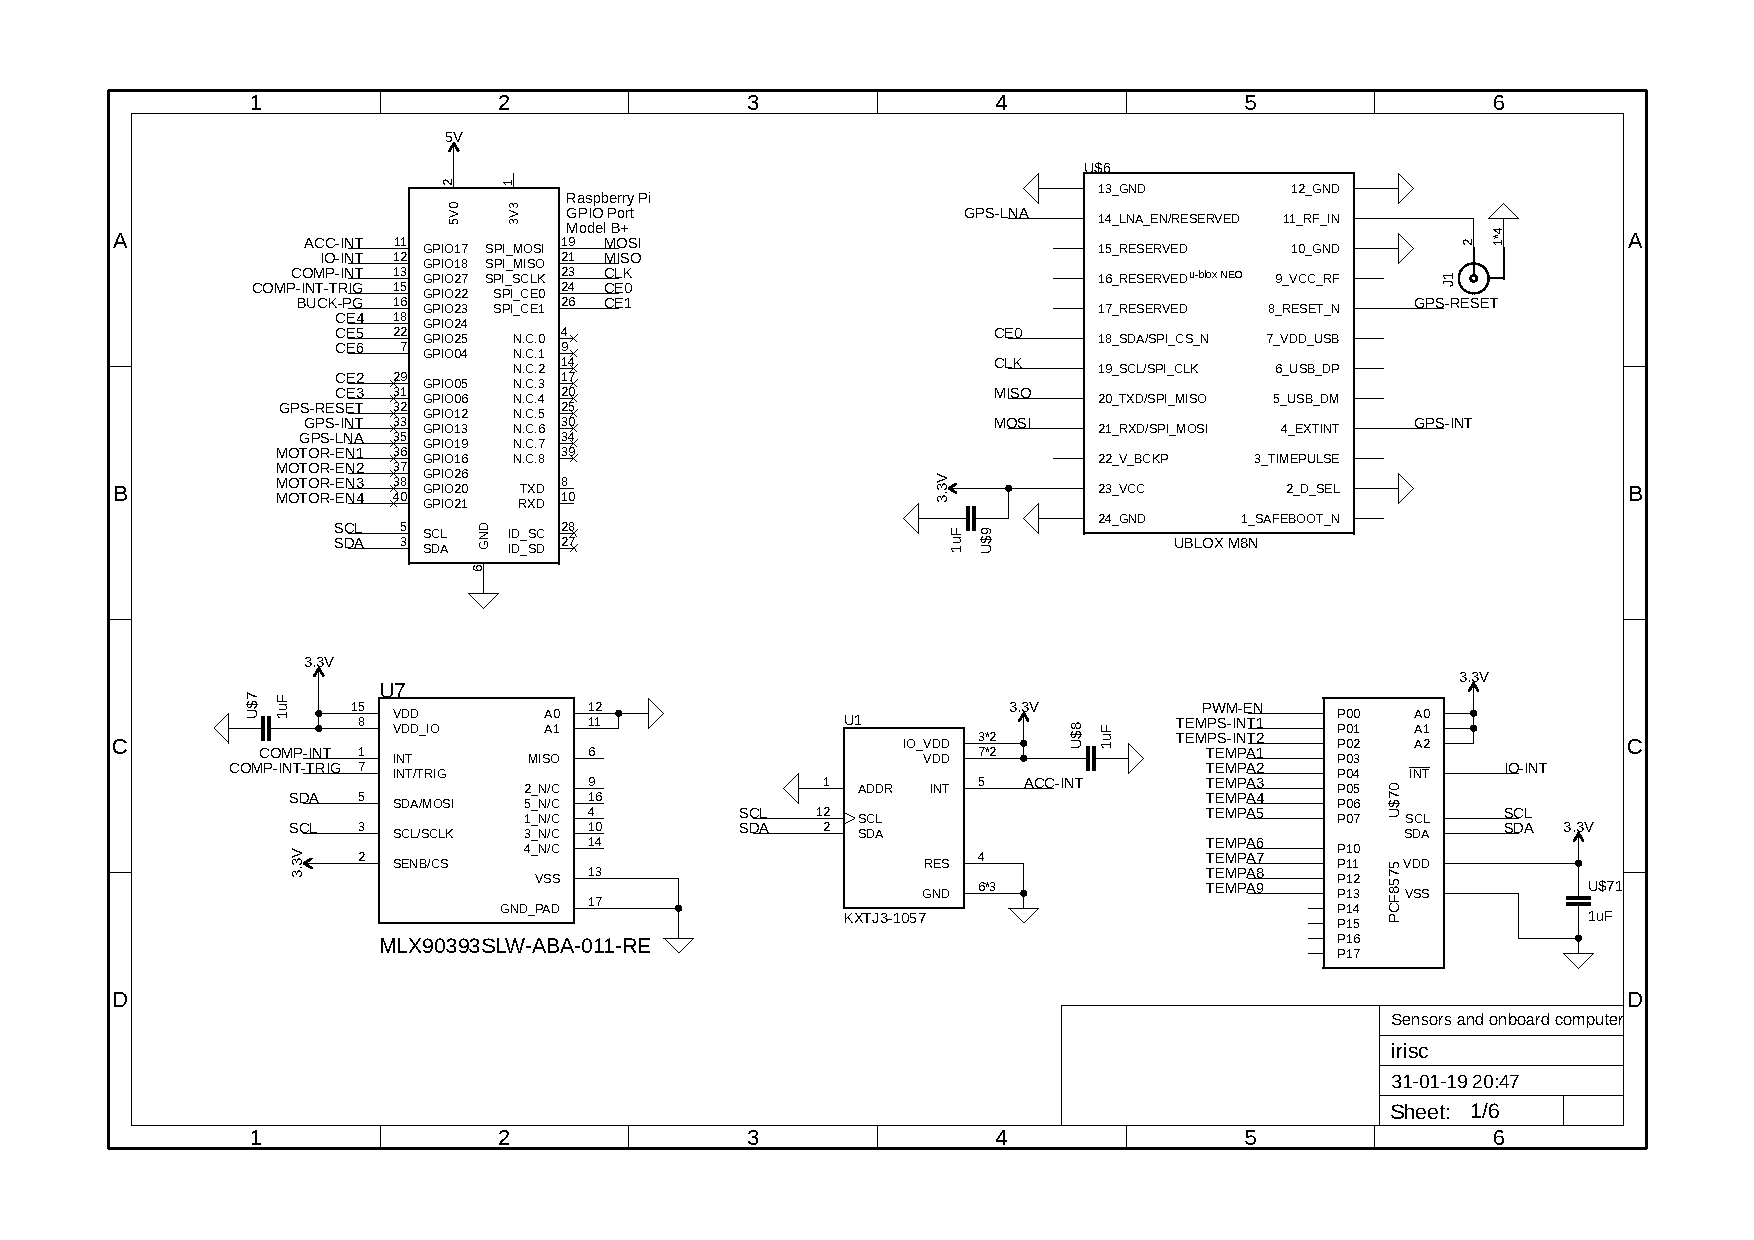
\includepdf [pages=1, angle=90]{appendix/img/schematics/irisc_v2.pdf}
\end{figure}
\newpage
\begin{figure}[h!]
		\includepdf [pages=2, angle=90]{appendix/img/schematics/irisc_v2.pdf}
\end{figure}
\newpage
\begin{figure}[h!]
		\includepdf [pages=3, angle=90]{appendix/img/schematics/irisc_v2.pdf}
\end{figure}
\newpage
\begin{figure}[h!]
		\includepdf [pages=4, angle=90]{appendix/img/schematics/irisc_v2.pdf}
\end{figure}
\newpage
\begin{figure}[h!]
		\includepdf [pages=5, angle=90]{appendix/img/schematics/irisc_v2.pdf}
\end{figure}
\newpage
\begin{figure}[h!]
		\includepdf [pages=6, angle=90]{appendix/img/schematics/irisc_v2.pdf}
\end{figure}

\newpage
\subsection{PCBs 1st iteration}
\begin{figure}[h!]
		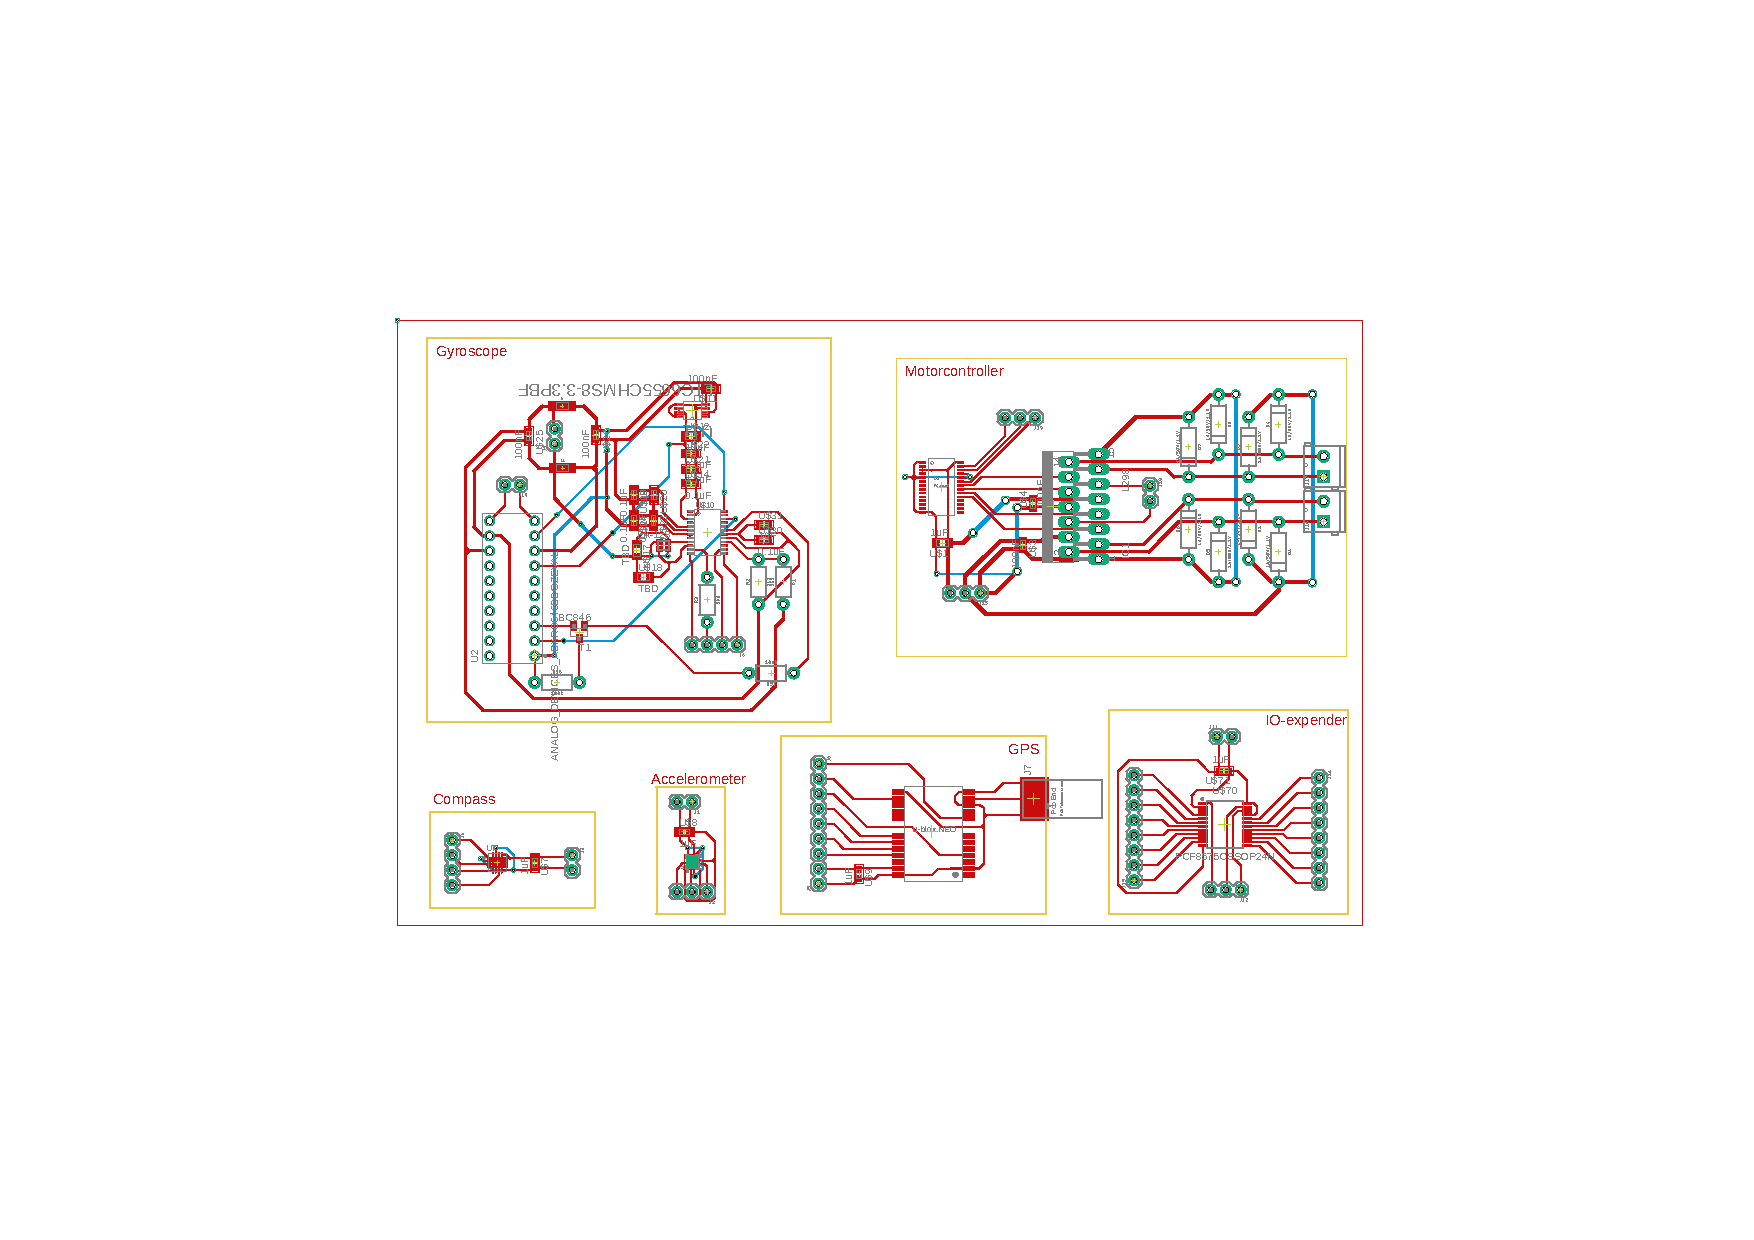
\includepdf [pages=1, angle=90]{appendix/img/pcb/irisc.pdf}
\end{figure}
\end{landscape}


\subsection{PCBs 2nd iteration}


% Highly recommend using the input function when you have a lot of stuff, it makes debugging and changing what appear in the appendix so much easier. It's also easier to edit and read. When your document starts to get big this will be the best decision you made ^^ 


% \subsection{Materials Properties}

% \input{4-experiment-design/tables/profile_material.tex}
% \bigskip
% \input{4-experiment-design/tables/wall_aluminum.tex}
% \bigskip
% \input{4-experiment-design/tables/wall_styrofoam.tex}
% \newpage
\newpage
\subsection{Manufacturing Drawings and Sketches}
\label{sec:mech_drawings}
% \begin{figure}[h!] 
% 		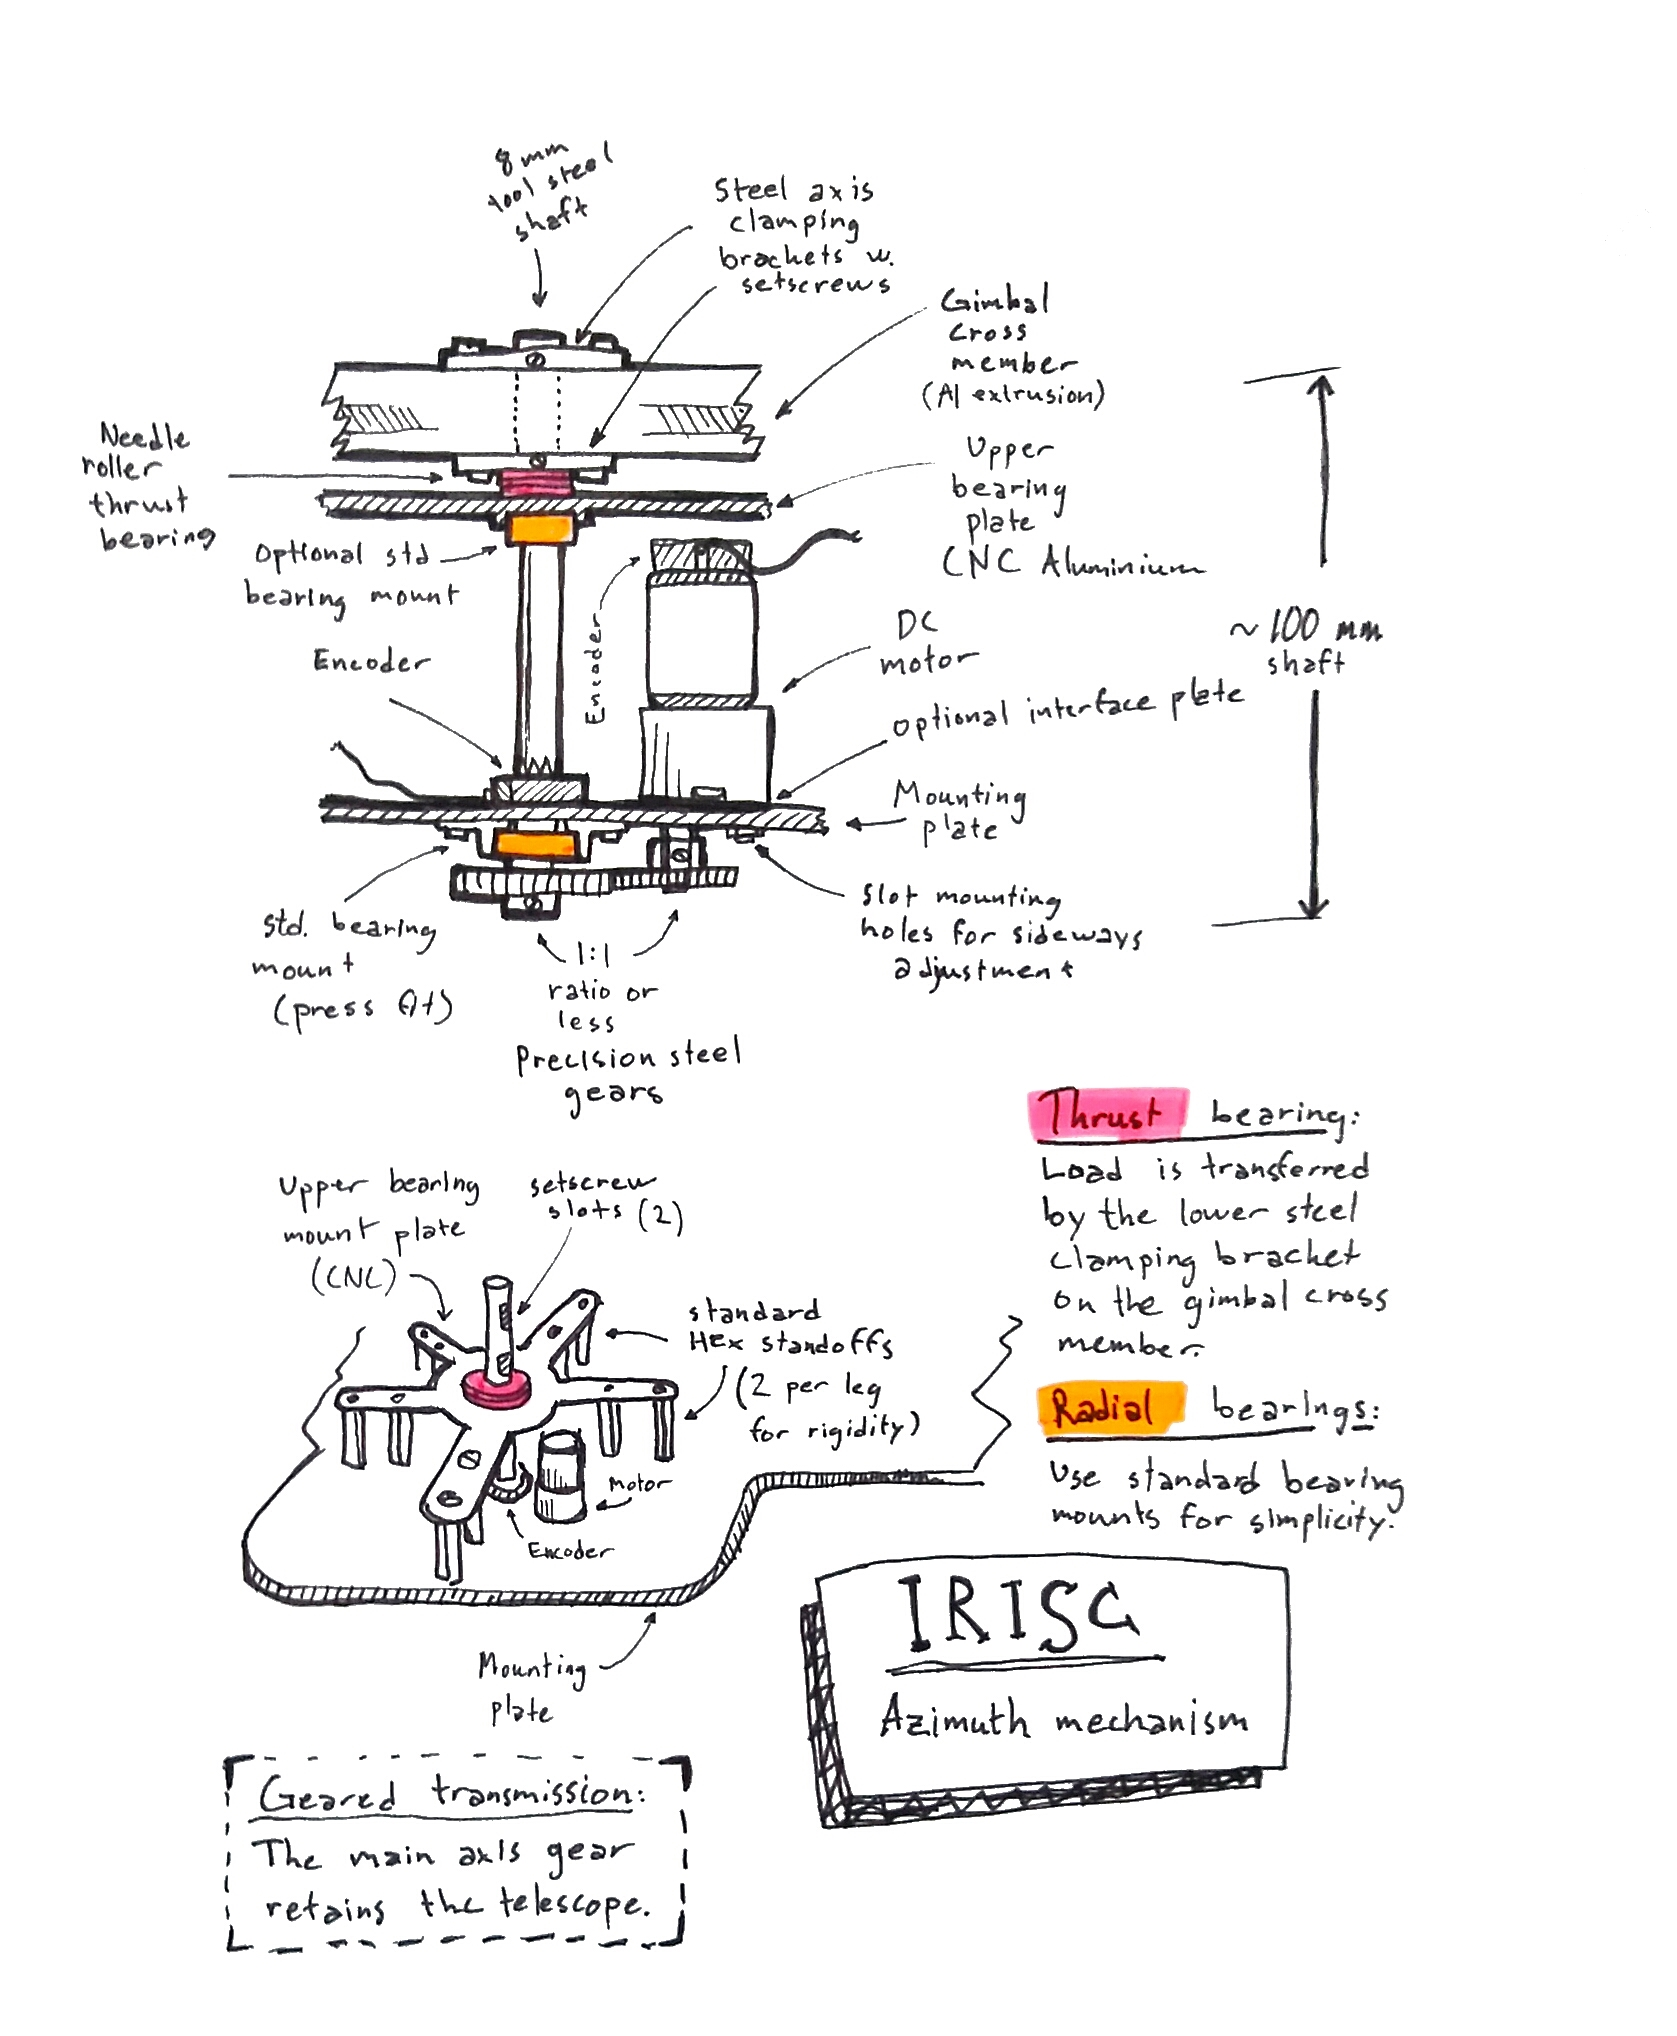
\includegraphics[width=\textwidth]{appendix/img/mechanical_sketches/azimuth_mechanism.jpg}
% 		\caption{Azimuth mechanism sketch.}
% 		\label{img:az_sketch}
% \end{figure}
% \newpage
% \begin{figure}[h!] 
% 		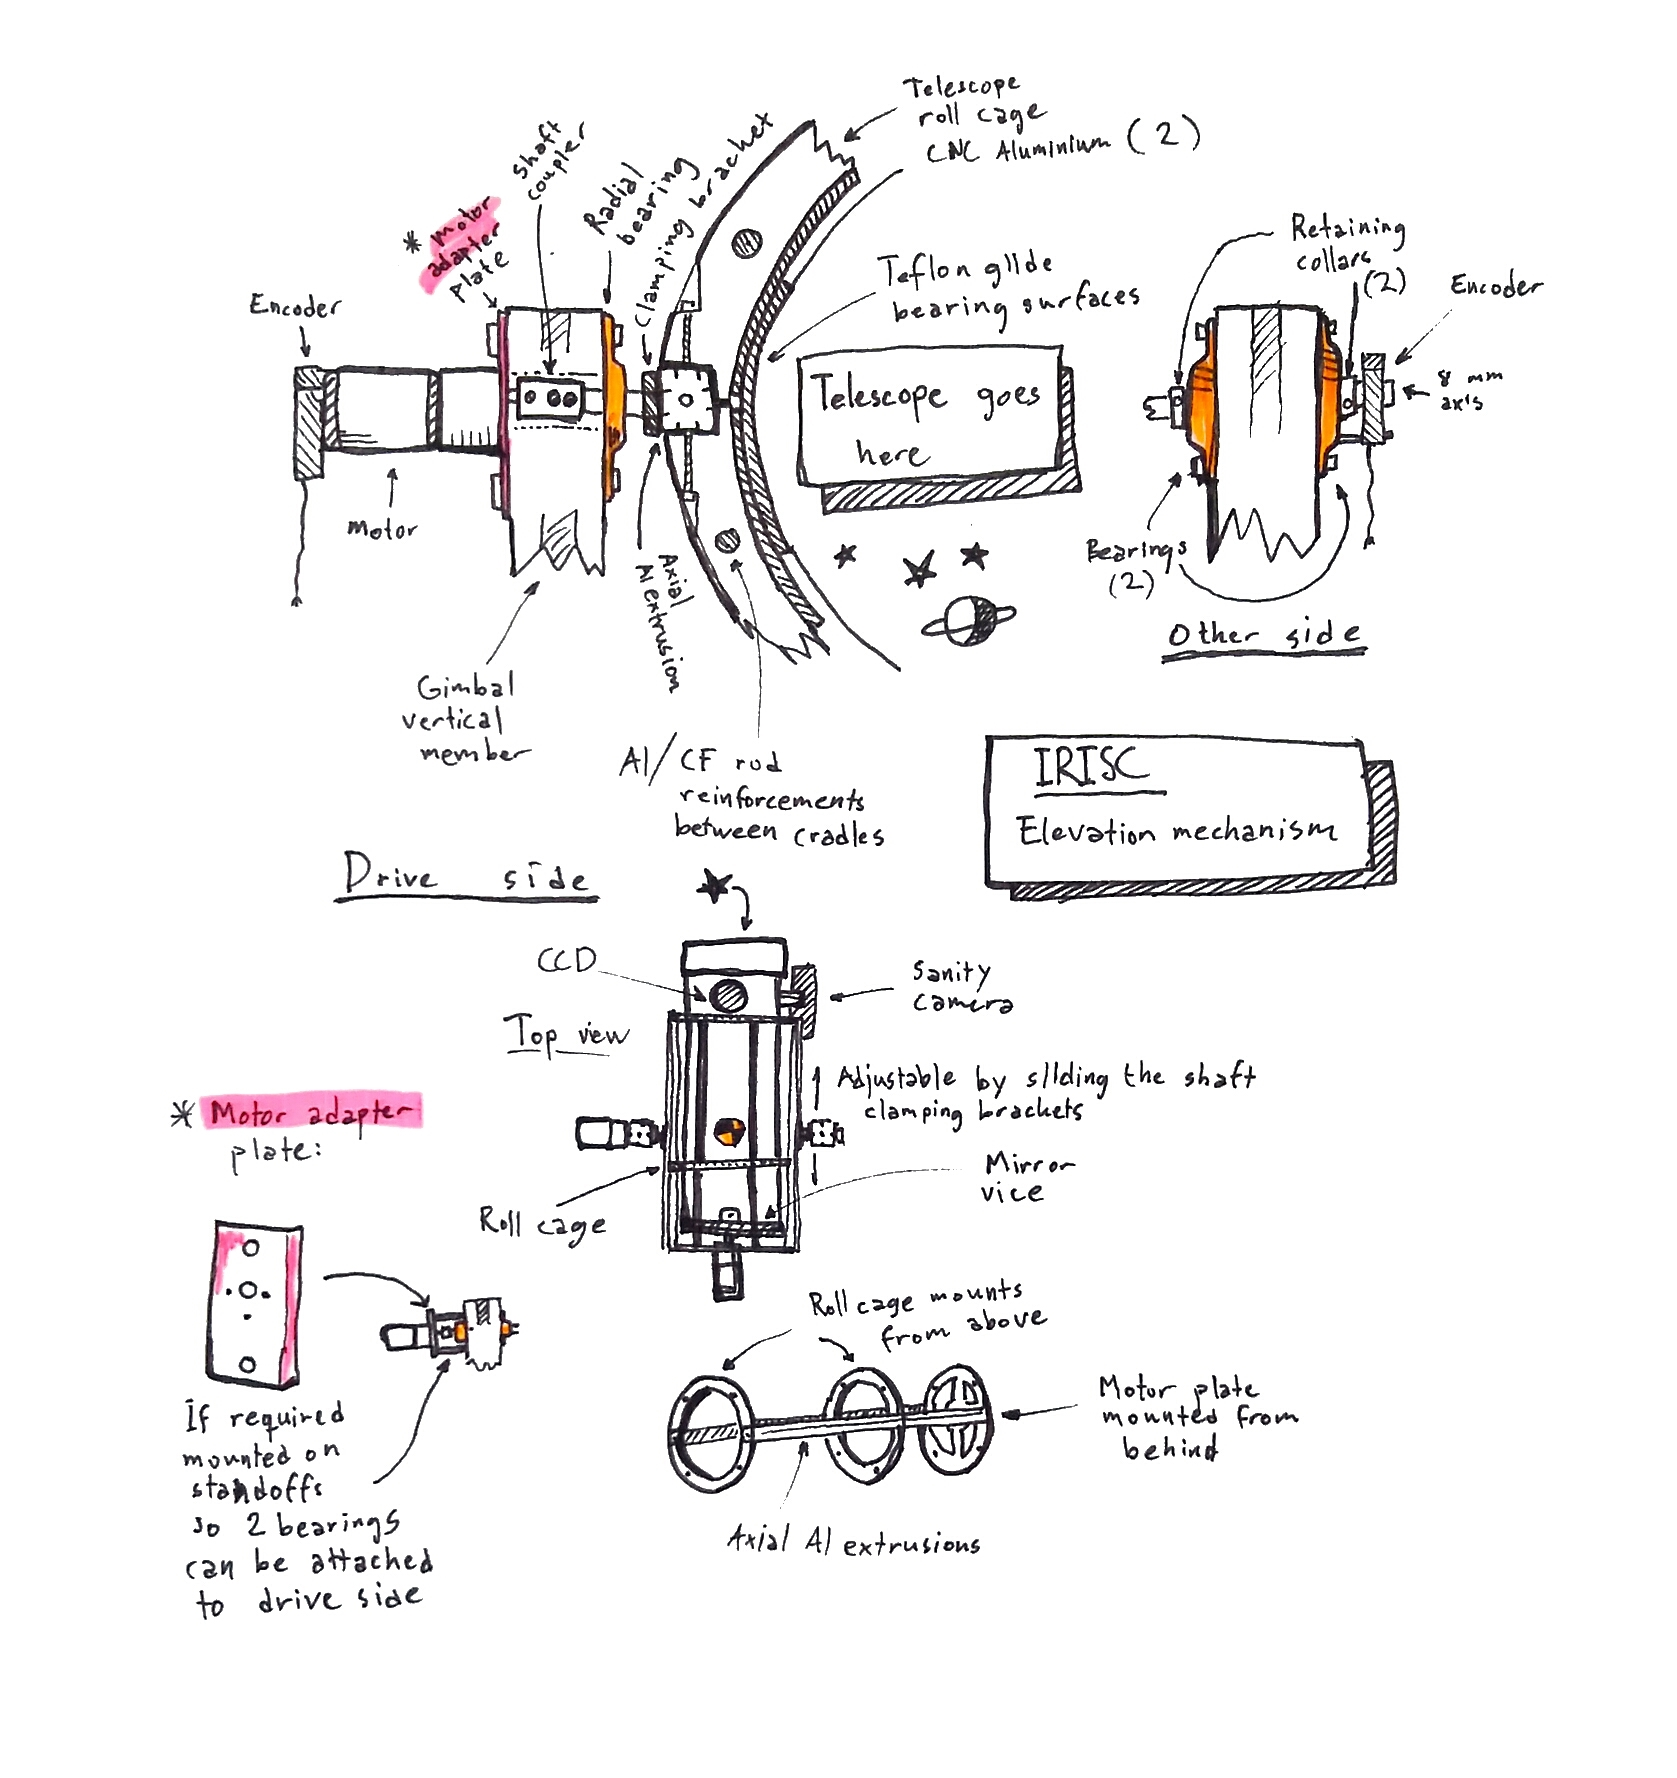
\includegraphics[width=\textwidth]{appendix/img/mechanical_sketches/elevation_mechanism.jpg}
% 		\caption{Elevation mechanism and roll cage sketch.}
% 		\label{img:el_sketch}
% \end{figure}
% \newpage
% \begin{figure}[h!] 
% 		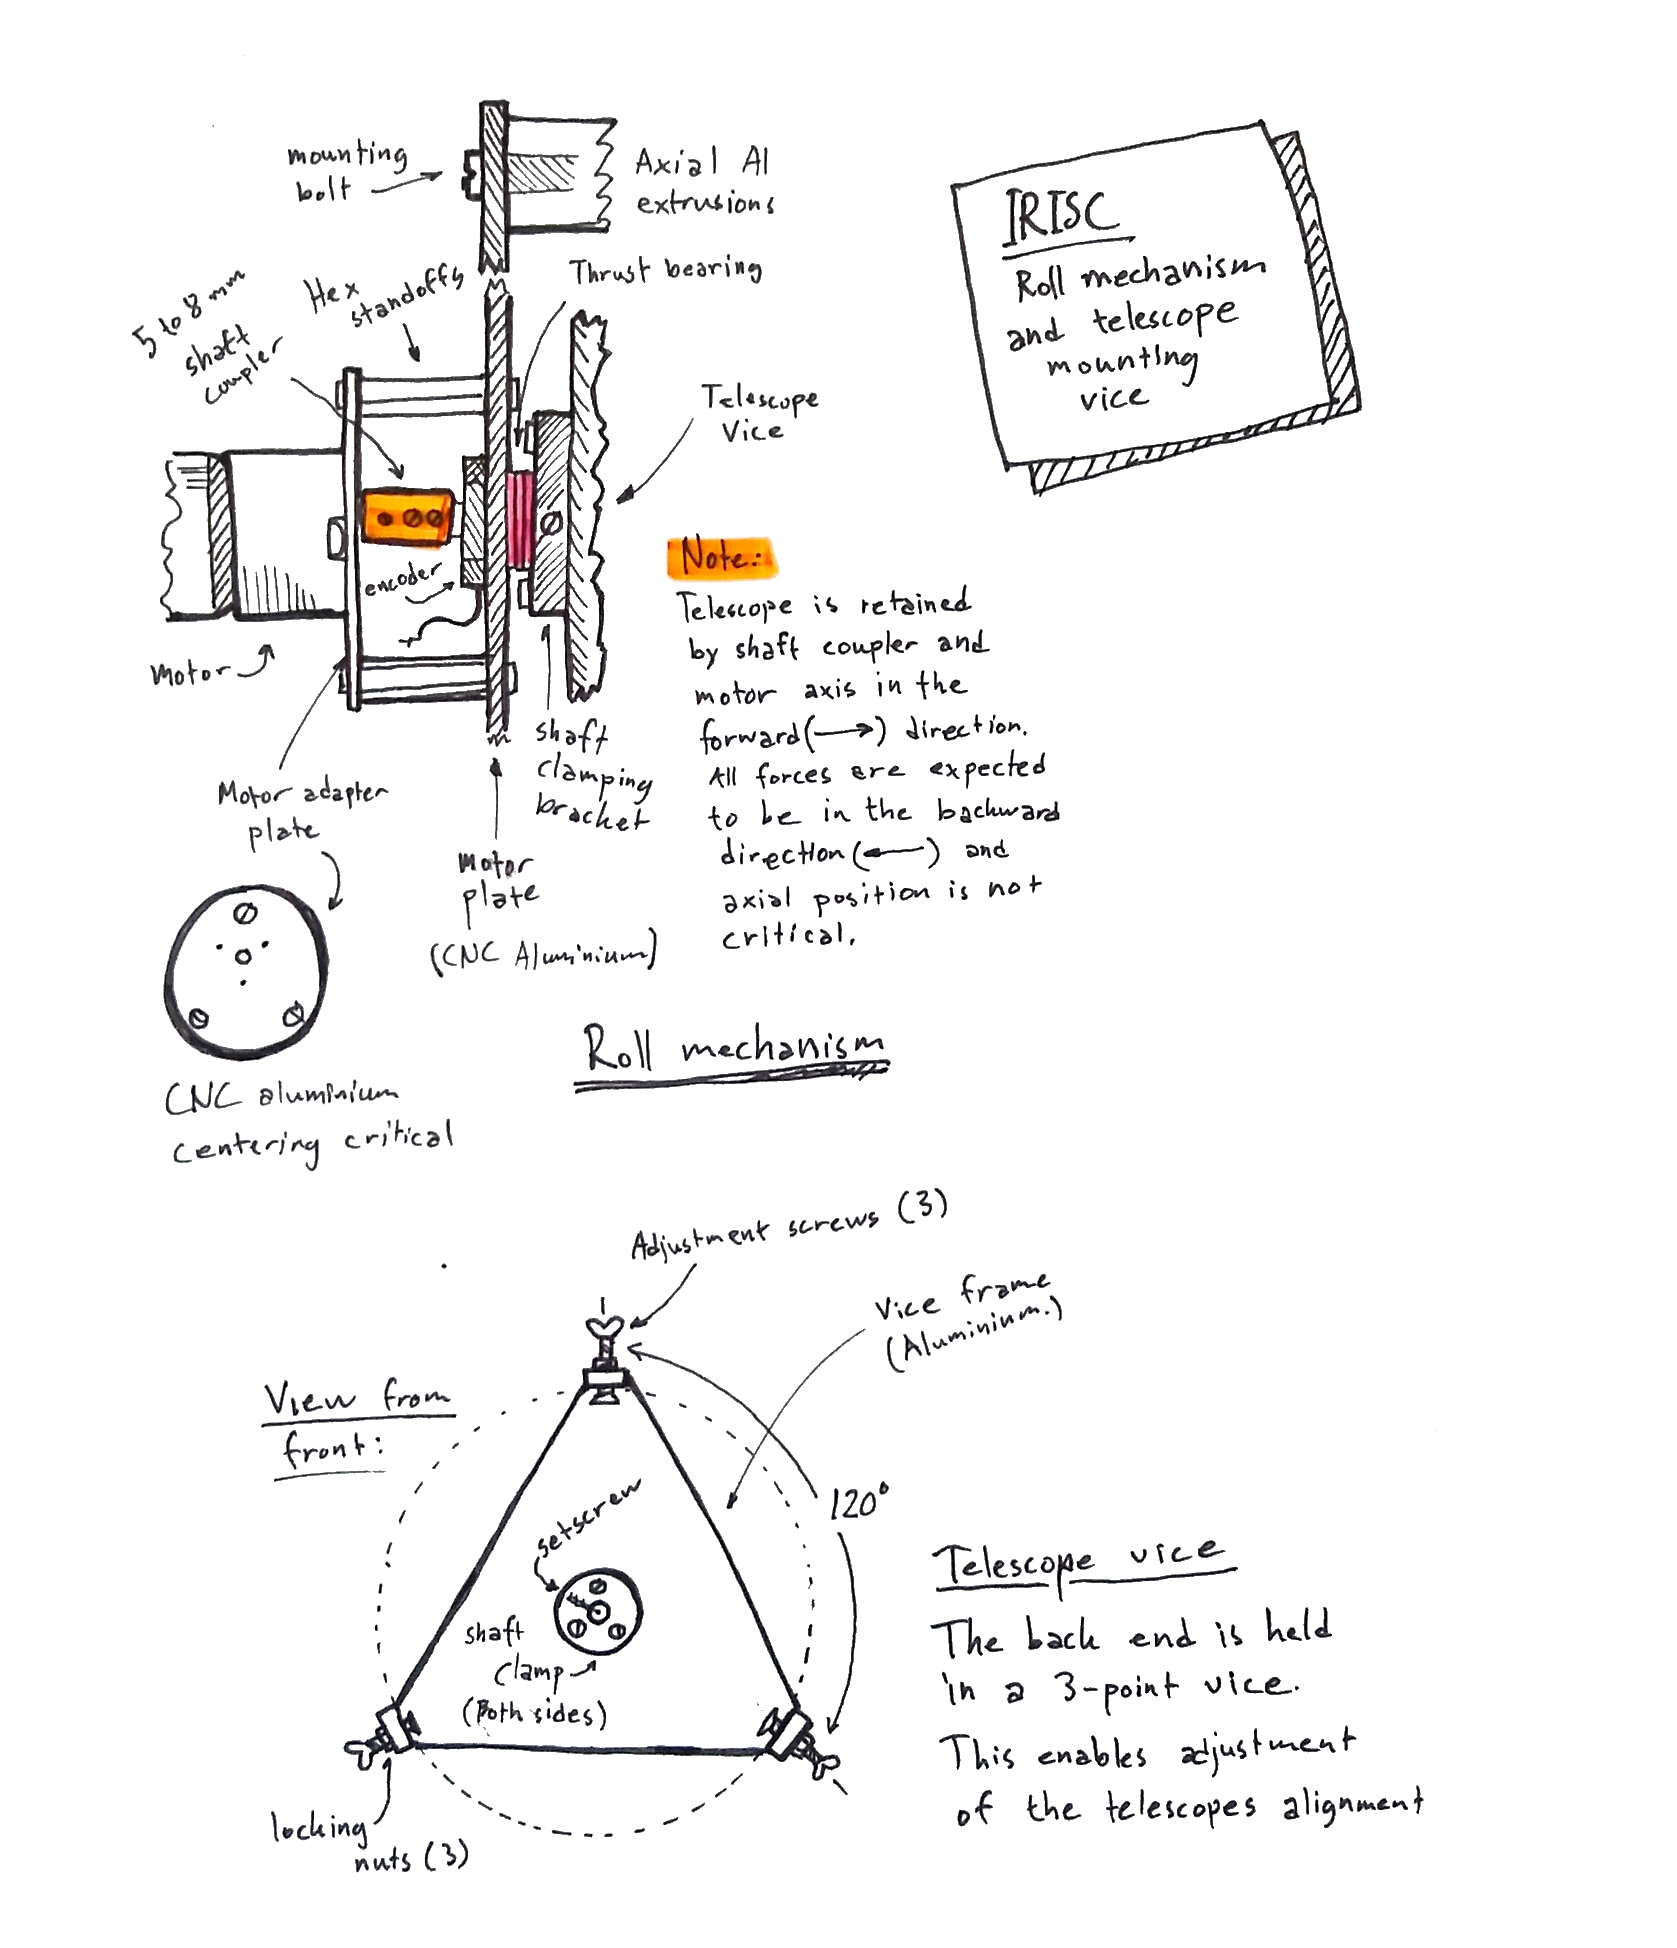
\includegraphics[width=\textwidth]{appendix/img/mechanical_sketches/roll_mechanism.jpg}
% 		\caption{Roll mechanism and telescope retaining vice sketch.}
% 		\label{img:roll_sketch}
% \end{figure}

\begin{figure}[H]
	\centering 
	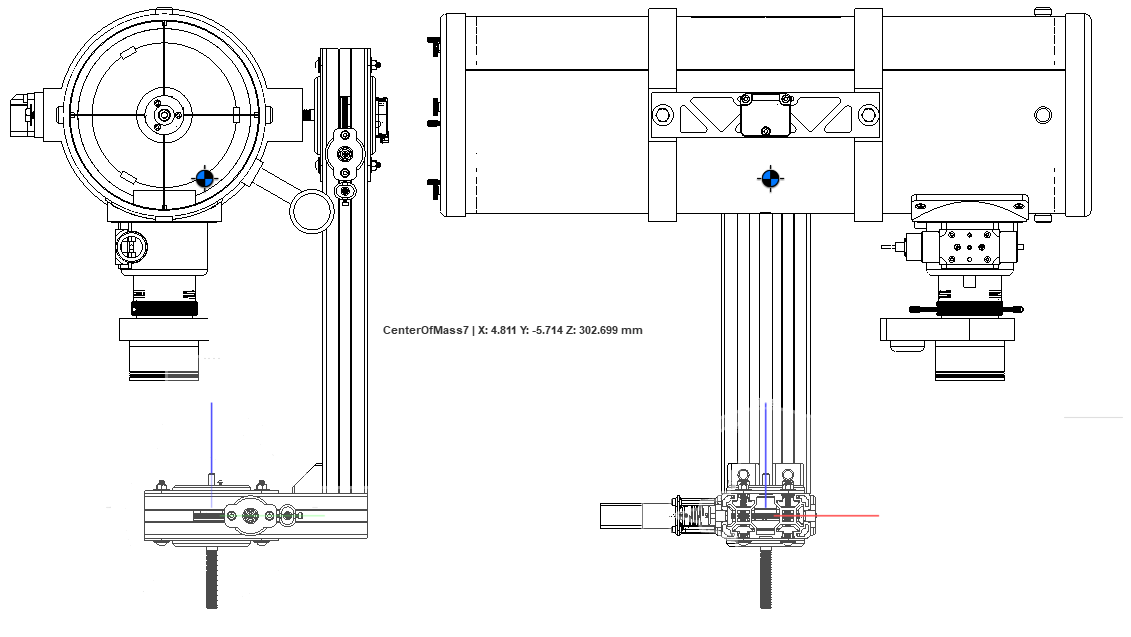
\includegraphics[scale=0.6]{4-experiment-design/img/mechanical/COM.png}
	\caption{Gimbal center of mass estimation.}
	\label{fig::mechanical::COM}
\end{figure}

\begin{landscape}
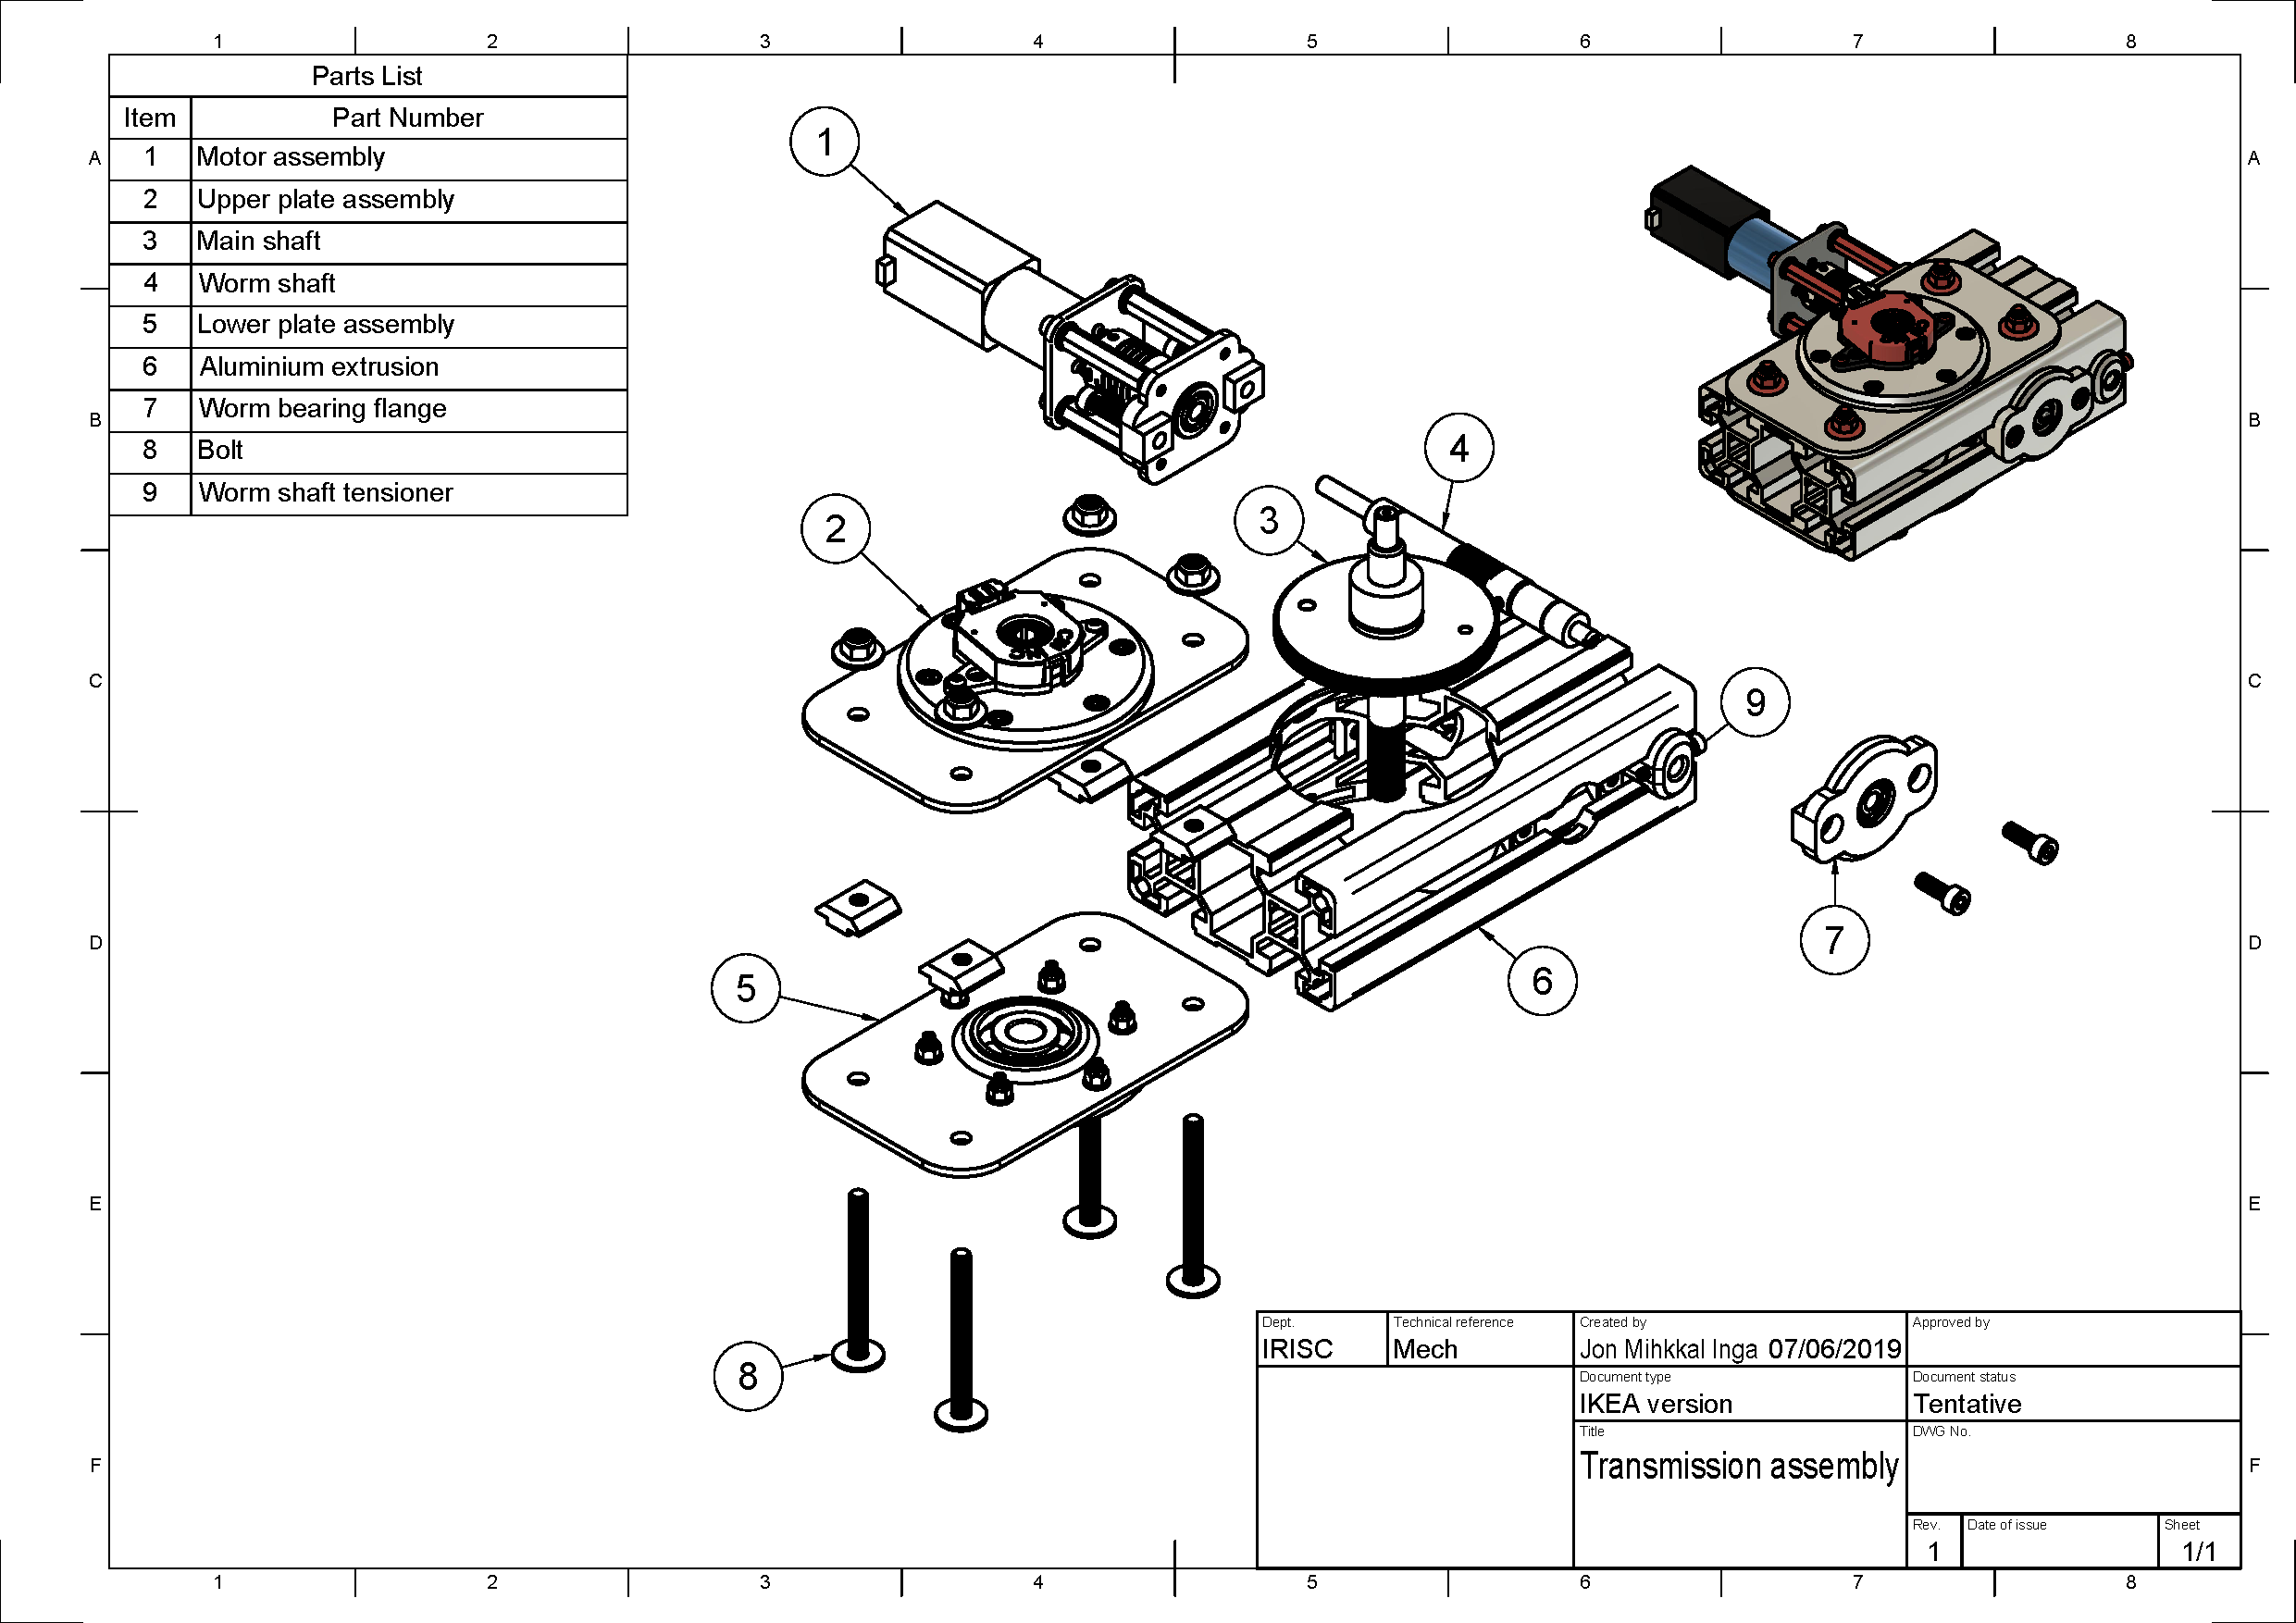
\includegraphics[scale=0.5]{appendix/img/mechanical_sketches/Transmission_Assembly.pdf}

\includegraphics[scale=0.5]{appendix/img/mechanical_sketches/Moments v1.pdf}

\end{landscape}
\newpage
% \includepdf[scale=1,pages={1,2,3,4,5,6,7,8,9,10,11,12,13,14,15,16,17,18,19,20,21,22,23,24,25,26,27,28,29,30,31,32,33,34,35,36}]{appendix/pdf/manufacturing-drafts.pdf}



% \newpage
% %\appendix
\begin{landscape}
\subsection{Software Sequence Diagram} \label{sec:XXX}

% \subsubsection{Air Sampling Control Object Sequence diagrams}
% \begin{figure}[H]
%     \centering
%     \includegraphics[height=0.9\textwidth]{appendix/img/softwareDiagrams/Sequance-Diagram-descent-Mode.jpg}
%     \caption{Sensor Object in Normal - Descent Mode.}
%     \label{sensorc}
% \end{figure}
\end{landscape}
% \newpage
% \subsection{Software Interface Diagram} \label{sec:XXXX}
% \subsubsection{Sensor Object Interface Diagram} %\label{}
% \begin{figure}[H]
%     \begin{align*}
%       \includegraphics[width=1\linewidth]{appendix/img/softwareDiagrams/interface_diagram-1-2.jpg}
%     \end{align*}
%     \caption{Sensor Object Interface Diagram.}
%     \label{fig:C1}
% \end{figure}


% \newpage
% \subsection{PCB Schematics}
\label{sec:pcbSchematics}

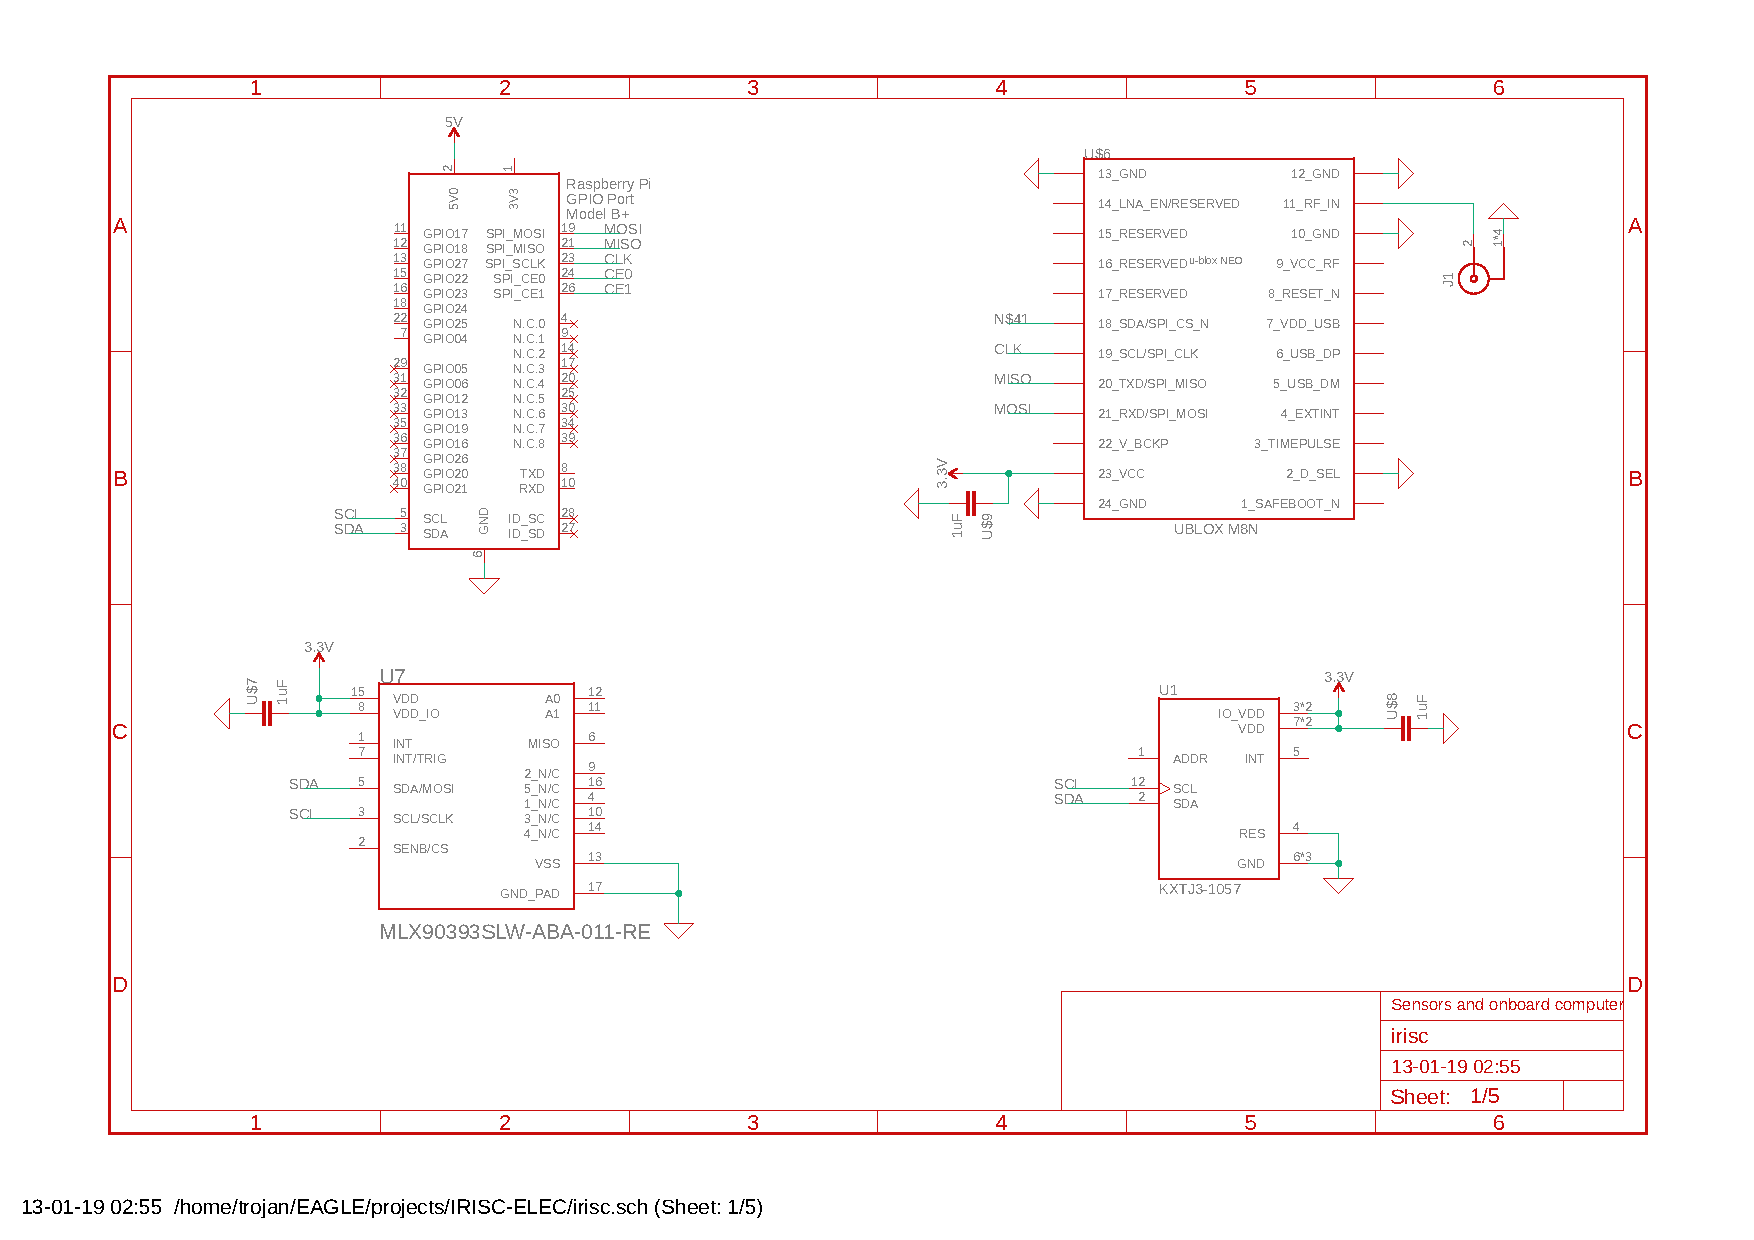
\includepdf[pages=-]{appendix/img/schematics/irisc.pdf}
% \newpage


% Same as with the experiment review PDFs but this time for data sheets of main/critical components


% \includepdf[scale=0.75,pages={3},pagecommand=\subsection{Tube}]{appendix/pdf/Rtx-Catalog015-6_Tubing.pdf}

% \includepdf[scale=0.75,pages={4},pagecommand=\subsection{AAC Manifold Valve}]{appendix/pdf/VDW_A_EU.pdf}
% \includepdf[scale=0.75,pages={7},pagecommand=\subsection{AAC Flushing Valve and CAC Valve}]{appendix/pdf/VDW_B_EU.pdf}
% \includepdf[scale=0.75,pages={8,9}]{appendix/pdf/VDW_B_EU.pdf}

% \includepdf[scale=0.75,pages={4},pagecommand=\subsection{Pump}]{appendix/pdf/DataSheet_NMP830_850_E005_web.pdf}

% \includepdf[scale=0.75,pages={1},pagecommand=\subsection{Airflow Sensor}]{appendix/pdf/honeywell-sensing-airflow-awm50000-series-catalog-pages.pdf}
% \includepdf[scale=0.75,pages={2,3,4}]{appendix/pdf/honeywell-sensing-airflow-awm50000-series-catalog-pages.pdf}

% \includepdf[scale=0.75,pages={1},pagecommand=\subsection{Static Pressure Sensor}]{appendix/pdf/Gems_3500_eng_tds.pdf}
% \includepdf[scale=0.75,pages={2,3}]{appendix/pdf/Gems_3500_eng_tds.pdf}